% Ubah judul dan label berikut sesuai dengan yang diinginkan.
\section{Architecture}
\label{sec:architecture}

\begin{enumerate}[label=\Alph*.]
    \item System Block Diagram
    \label{subsec:systemblockdiagram}

    \hspace*{1em} The designed system has several main components: sensors, control, mechanical system, and motion data. The sensor part includes load cells on each robot's sole to detect loads and maintain balance. The control part involves a microcontroller that processes sensor data and controls the robot's movements. The mechanical system includes the robot's frame with various servos to move the robot. The motion data part stores the designed movements in the microcontroller's file system, containing arrays of target servo positions and the time required to achieve them. The block diagram of the humanoid robot system can be seen in Figure \ref{fig:Diagram_Sistem}.

    \begin{figure} [h] \centering
        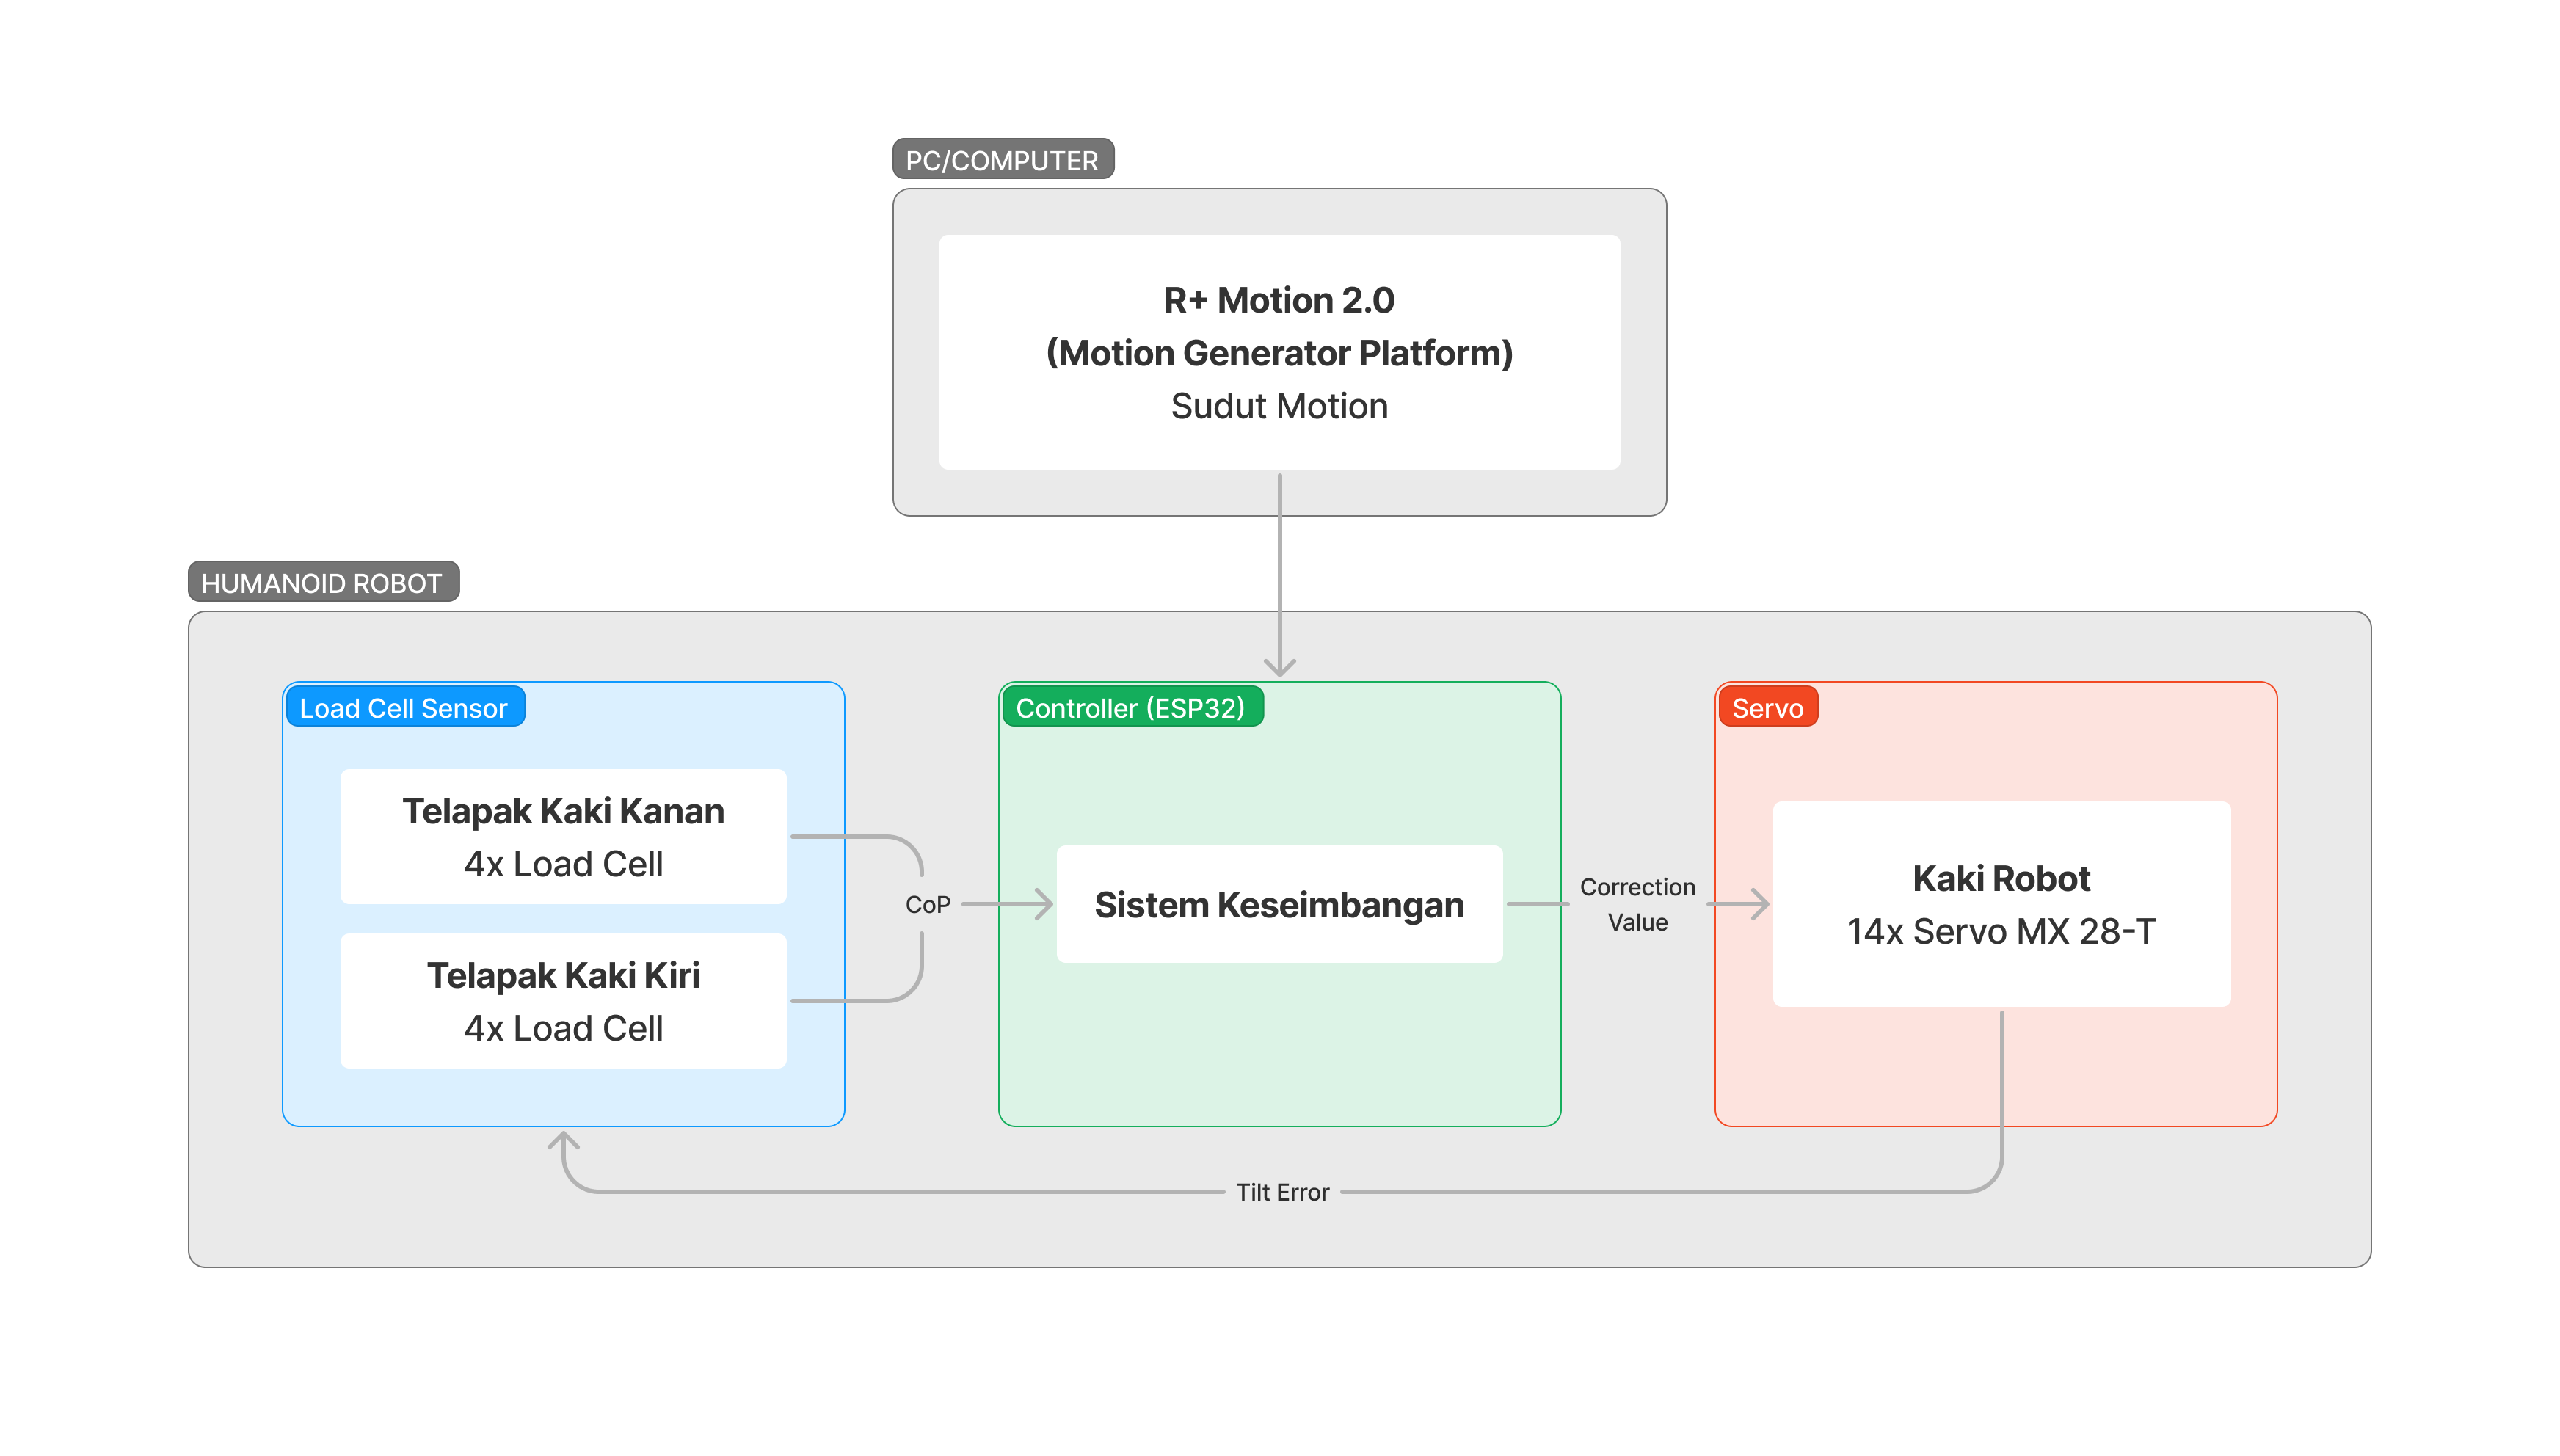
\includegraphics[width=0.45\textwidth]{gambar/Diagram_Sistem.png}
        \caption{System Diagram}
        \label{fig:Diagram_Sistem}
    \end{figure}

    \item Mechanical System
    \label{subsec:mechanicalsystem}

    \hspace*{1em} The design of this humanoid robot includes 29 servo motors. The upper body uses 15 XL-320 servos, while the lower body uses 14 MX-28 servos. The design details, sizes, and servo ID naming on the robot can be seen in Figure \ref{fig:Desain_Mekanik}. Information about the robot's degrees of freedom can be found in Table \ref{tab:DOF_Robot}, while the robot dimensions are listed in Table \ref{tab:Dimensi_Robot}.

    \begin{figure} [h] \centering
      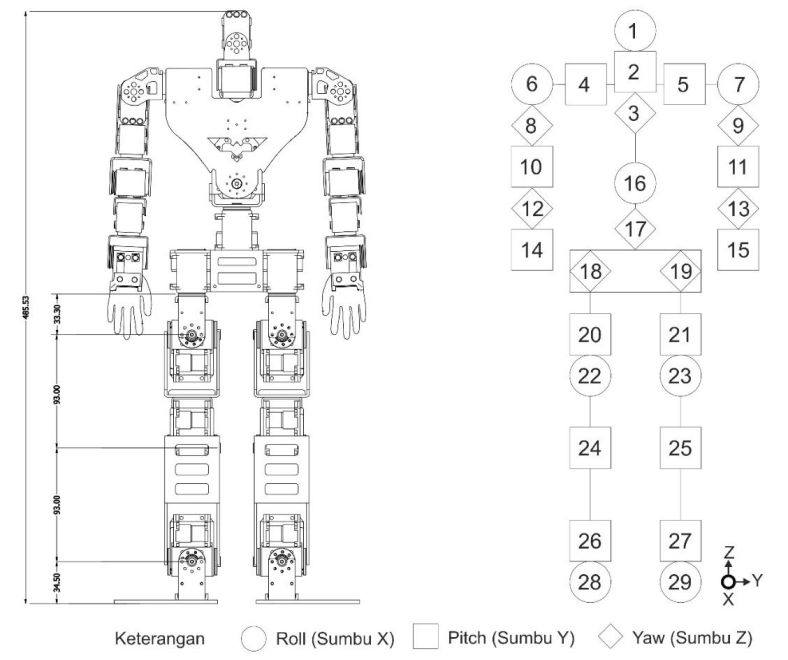
\includegraphics[width=0.35\textwidth]{gambar/Desain_Mekanik.png}
      \caption{Mechanical Design of the Robot}
      \label{fig:Desain_Mekanik}
    \end{figure}

    % Table for Degrees of Freedom (DOF)
    \begin{table}[htb]
      \centering
      \caption{Degrees of Freedom (DOF) of Body Parts}
      \begin{tabular}{>{\itshape}l >{\itshape}l >{\itshape}l}
        \toprule
        \textit{Body Part} & \textit{DOF} & \textit{Total} \\
        \midrule
        Head & 3 DOF & 3 \\
        Arm (Shoulder) & 2 DOF x 2 & 4 \\
        Arm (Elbow) & 2 DOF x 2 & 4 \\
        Arm (Hand/Wrist) & 2 DOF x 2 & 4 \\
        Torso & 2 DOF & 2 \\
        Leg (Hip) & 3 DOF x 2 & 6 \\
        Leg (Knee) & 1 DOF x 2 & 2 \\
        Leg (Ankle) & 2 DOF x 2 & 4 \\
        \midrule
        Total & & 29 \\
        \bottomrule
      \end{tabular}
      \label{tab:DOF_Robot}
    \end{table}

    % Table with Italic Text
    \begin{table}[h]
      \centering
      \caption{Robot Dimensions}
      \begin{tabular}{>{\itshape}l >{\itshape}l}
        \toprule
        \textit{Dimension} & \textit{Length (mm)} \\
        \midrule
        Height & 485 \\
        Width (Shoulder to Shoulder) & 116 \\
        Depth (Chest to Back) & 45 \\
        Length of Upper Leg & 124.5 \\
        Length of Lower Leg & 127.5 \\
        Length between hip joints & 73.8 \\
        Length of Upper Arm & 97 \\
        Length of Lower Arm & 128.5 \\
        Width of sole & 84.5 \\
        Length of sole & 135.5 \\
        \bottomrule
      \end{tabular}
      \label{tab:Dimensi_Robot}
    \end{table}

    \item Electronic System
    \label{subsec:electronicsystem}

    \hspace*{1em} The hardware system in this research is described through a block diagram shown in Figure \ref{fig:Diagram_Elektronik}. This system uses an embedded system consisting of an ESP32 and an ESP32-C3 microcontroller. The embedded system was chosen because the robot developed in this research is an improvement from previous research conducted by Fahd (2018). 

    \begin{figure} [h] \centering
      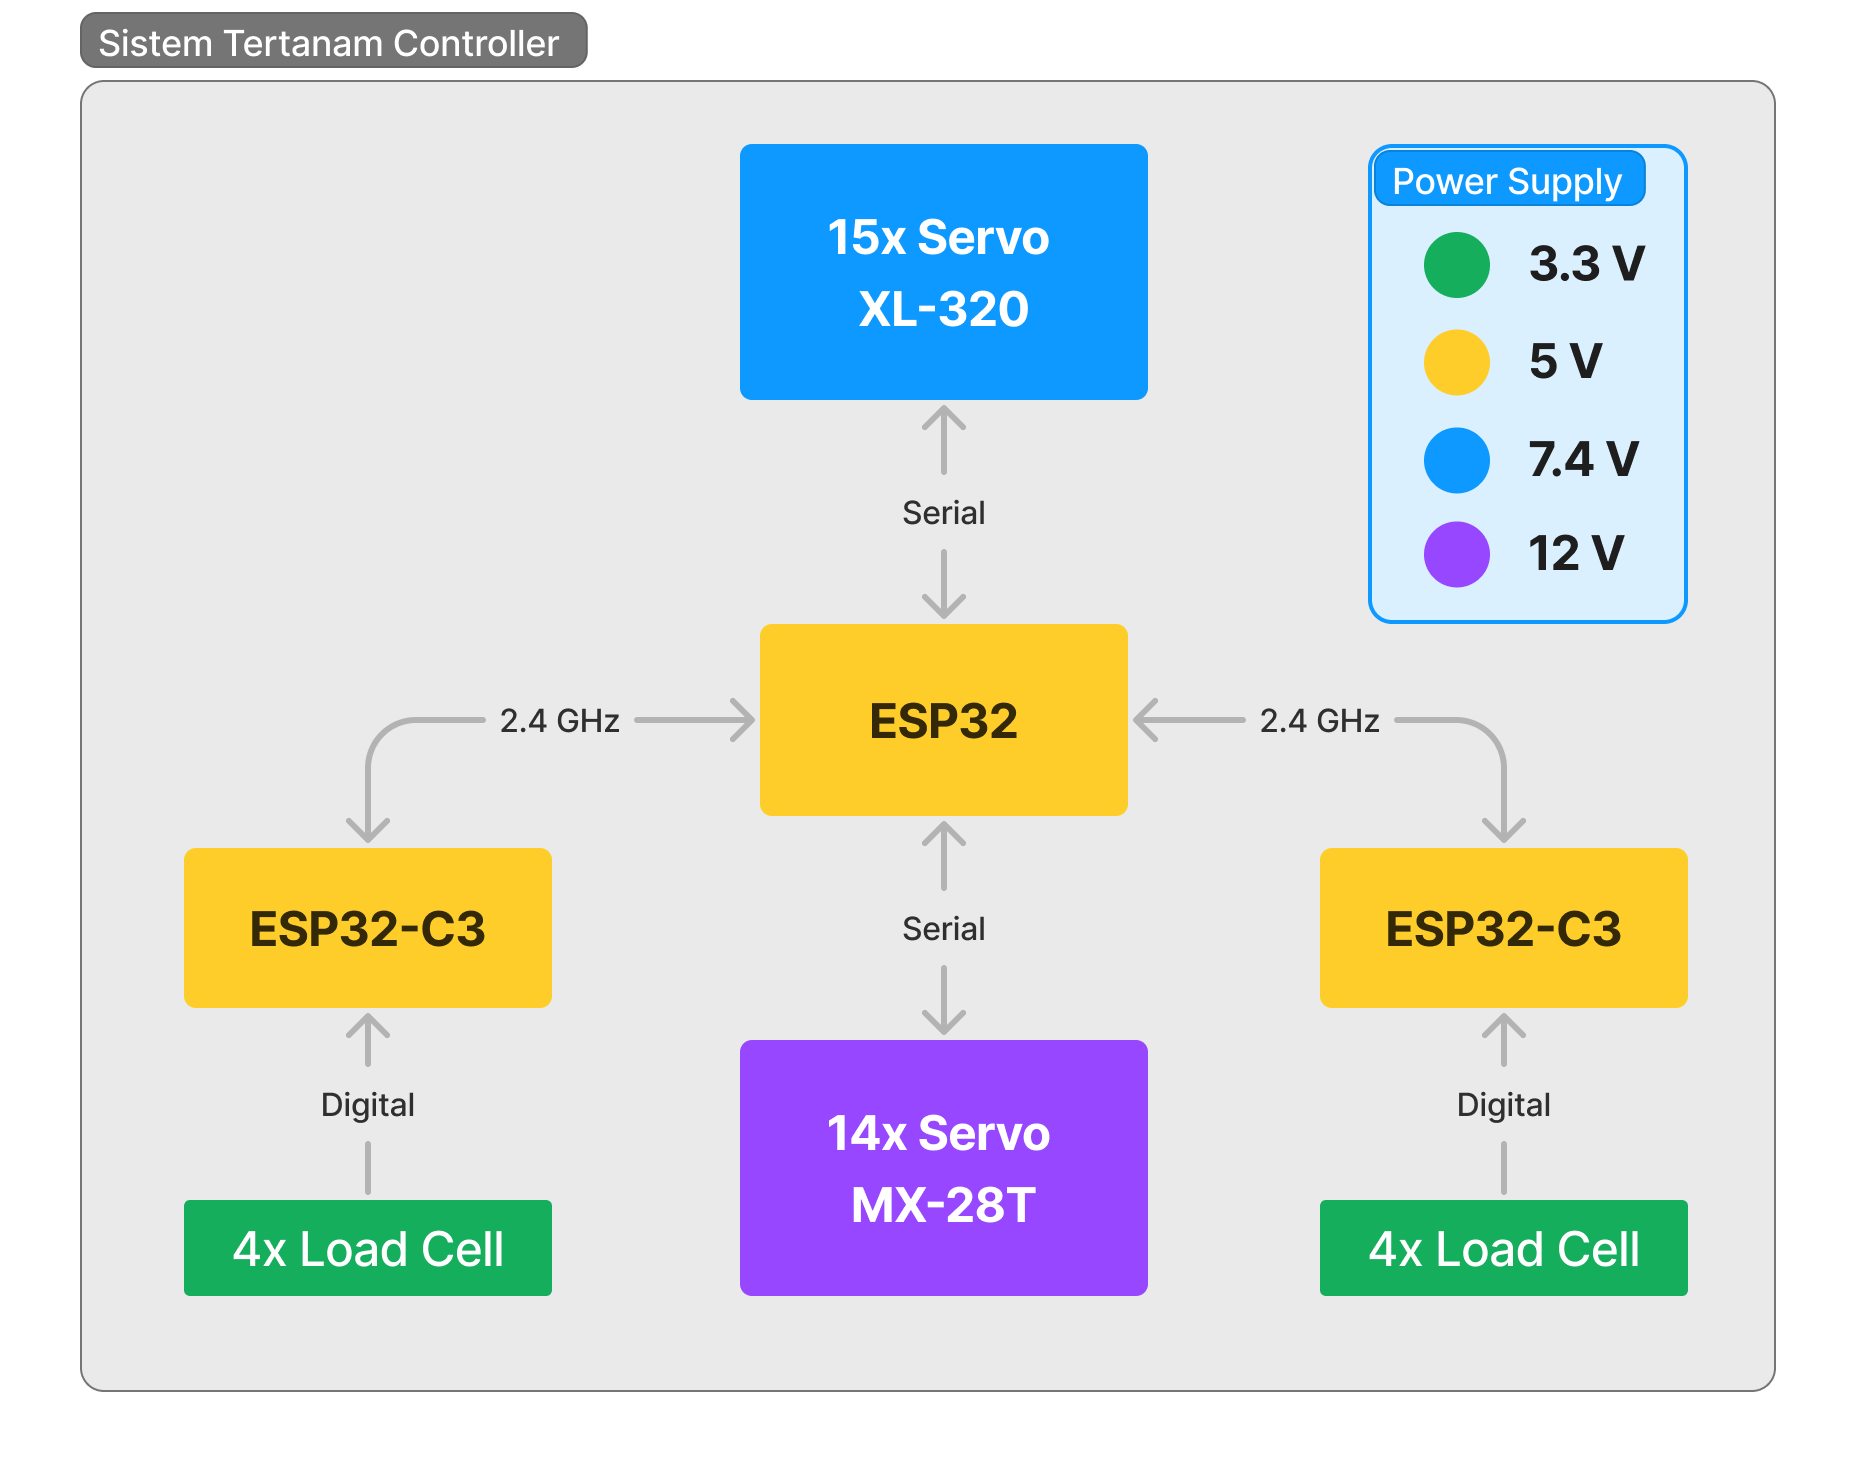
\includegraphics[width=0.4\textwidth]{gambar/Diagram_Elektronik.png}
      \caption{Electronic System Diagram}
      \label{fig:Diagram_Elektronik}
    \end{figure}

    \hspace*{1em} The ESP32-C3 is used for data acquisition from the load cells and sends it to the ESP32. The ESP32-C3 has the same Wi-Fi capability as the ESP32, allowing wireless communication between the two microcontrollers. The ESP32-C3 also has smaller dimensions, making it easier to place on the robot's legs. 

    \item Load Cell System Design
    \label{subsec:loadcellsystemdesign}

    \hspace*{1em} Each robot's sole is equipped with 4 load cells mounted at the ends of the feet. Each load cell detects pressure, allowing the system to determine the position of the center of pressure on the robot's sole. The design of the robot's sole can be seen in Figure \ref{fig:Dia_LoadCell}.

    \begin{figure} [h] \centering
        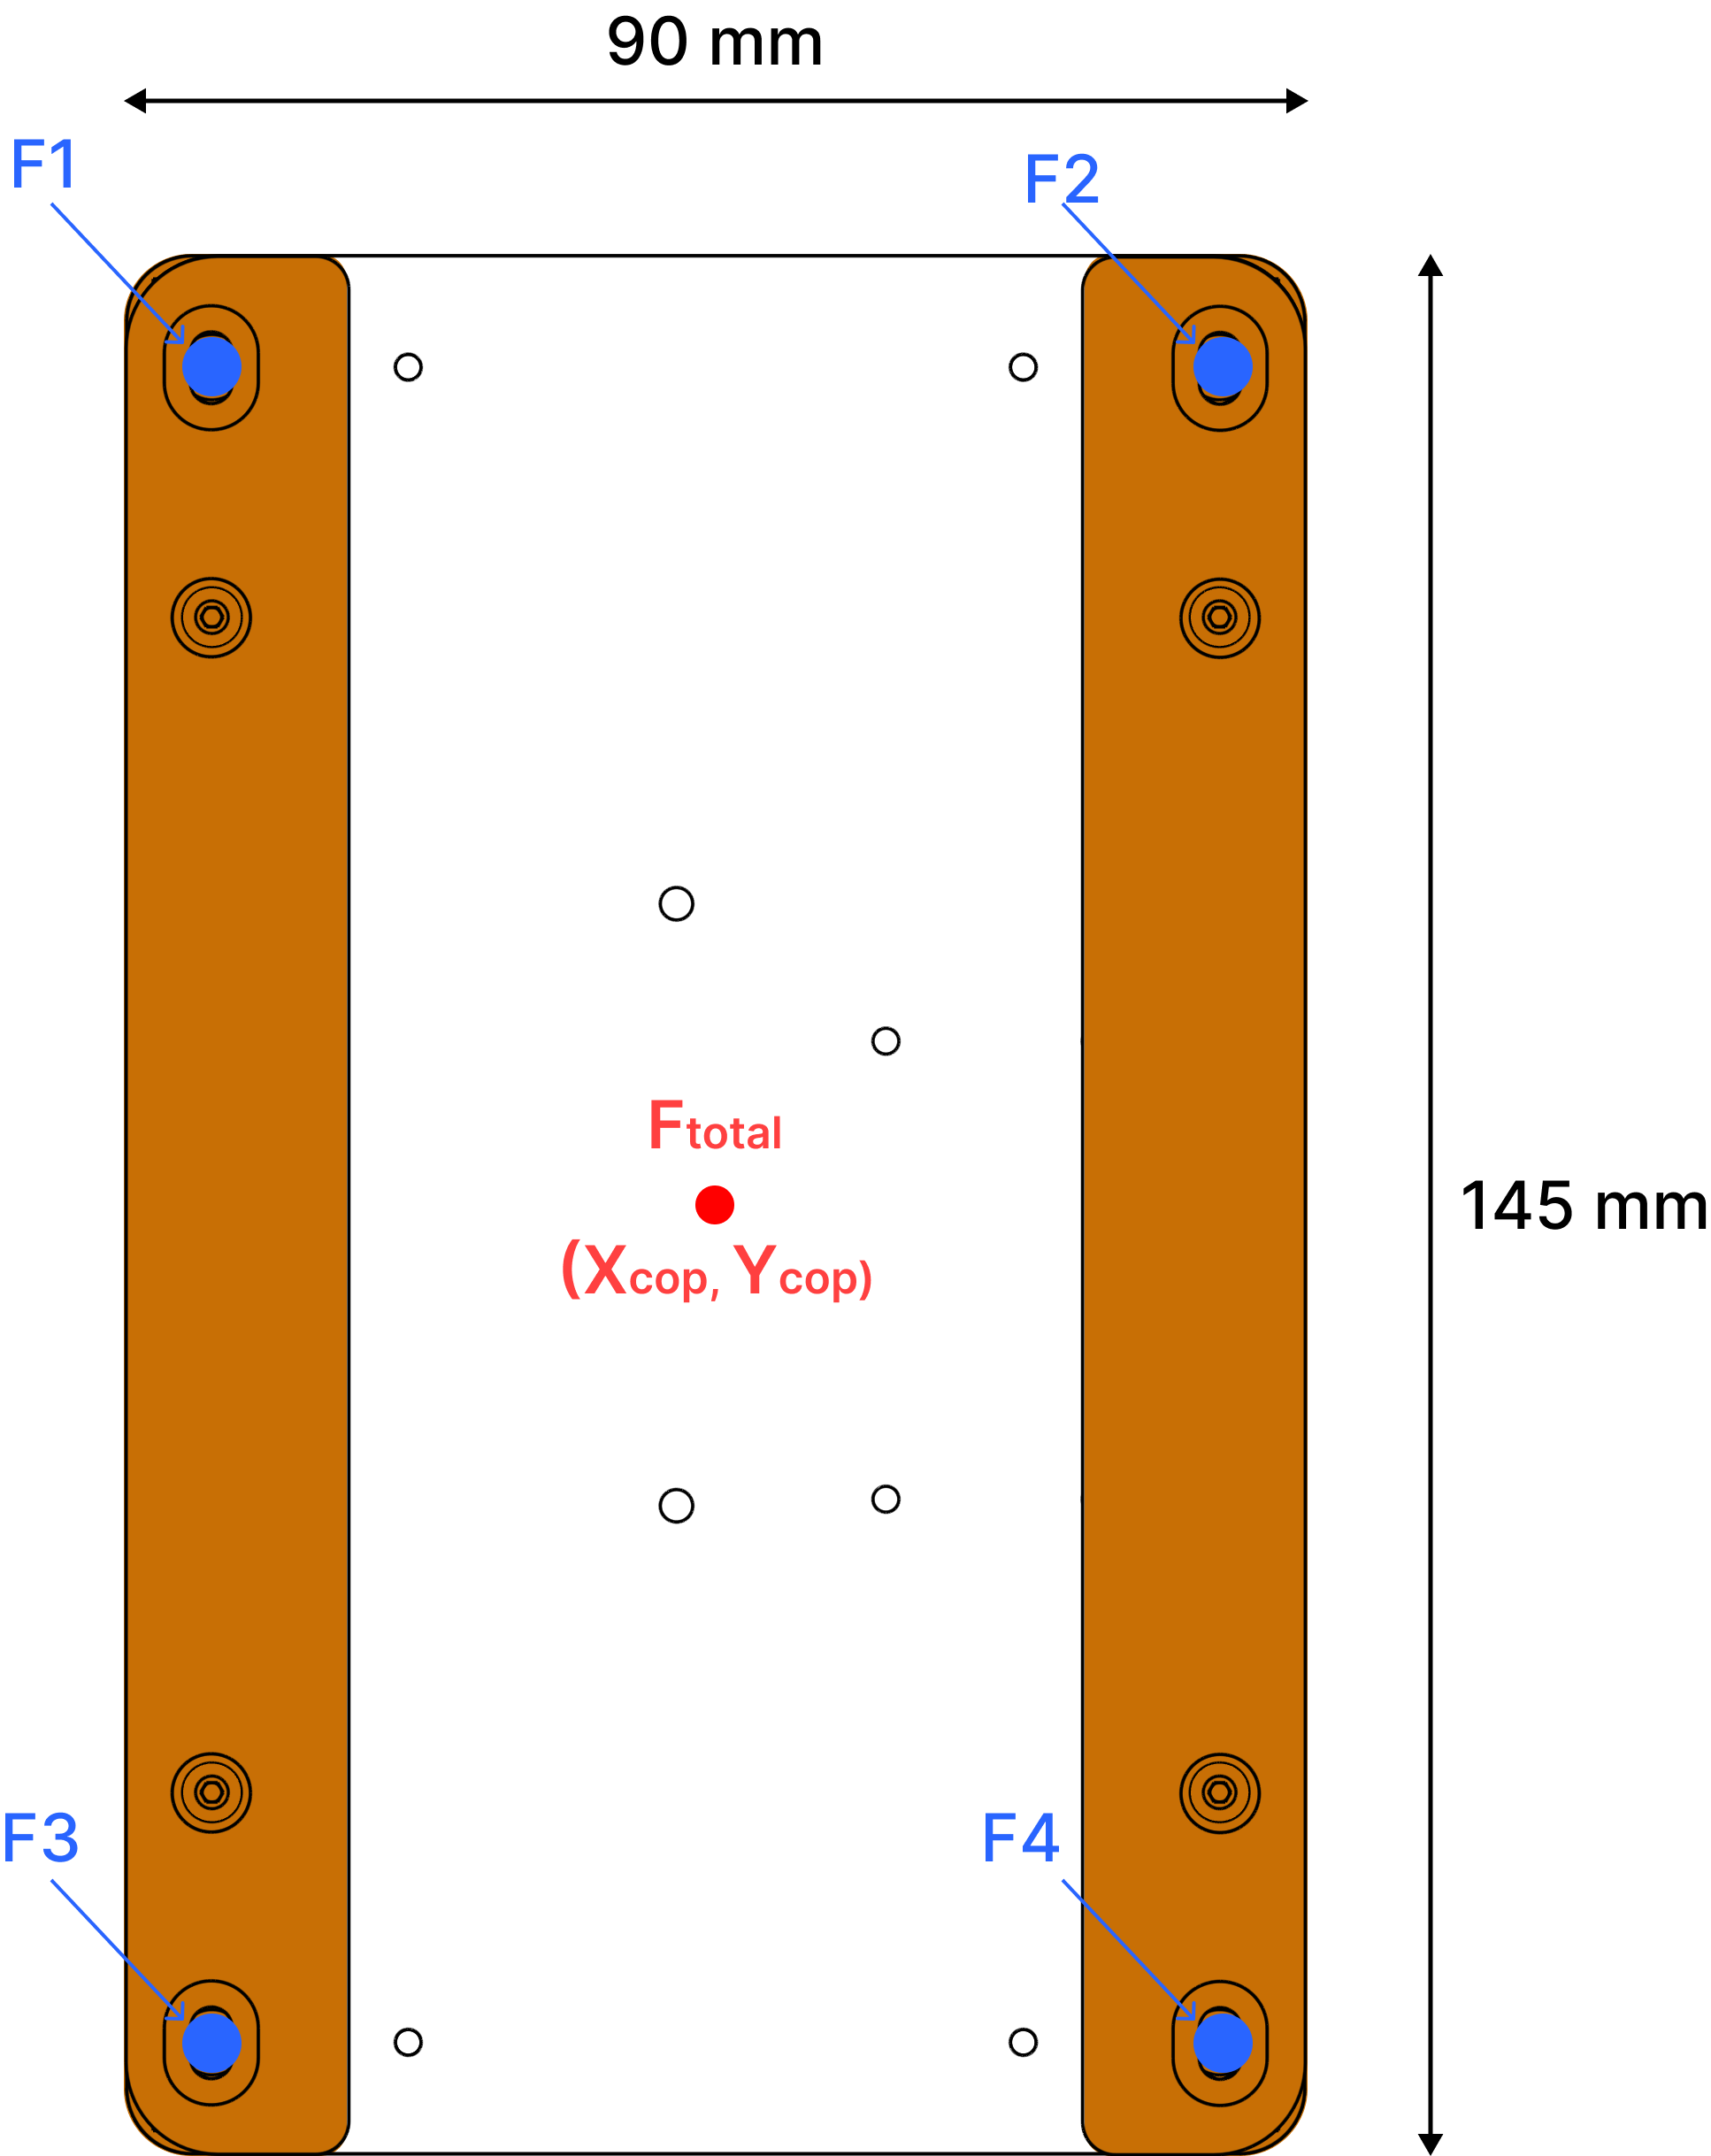
\includegraphics[width=0.3\textwidth]{gambar/Diagram_LoadCell.png}
        \caption{Load Cell Design on the Robot's Sole}
        \label{fig:Dia_LoadCell}
    \end{figure}
    
    \begin{figure} [h] \centering
      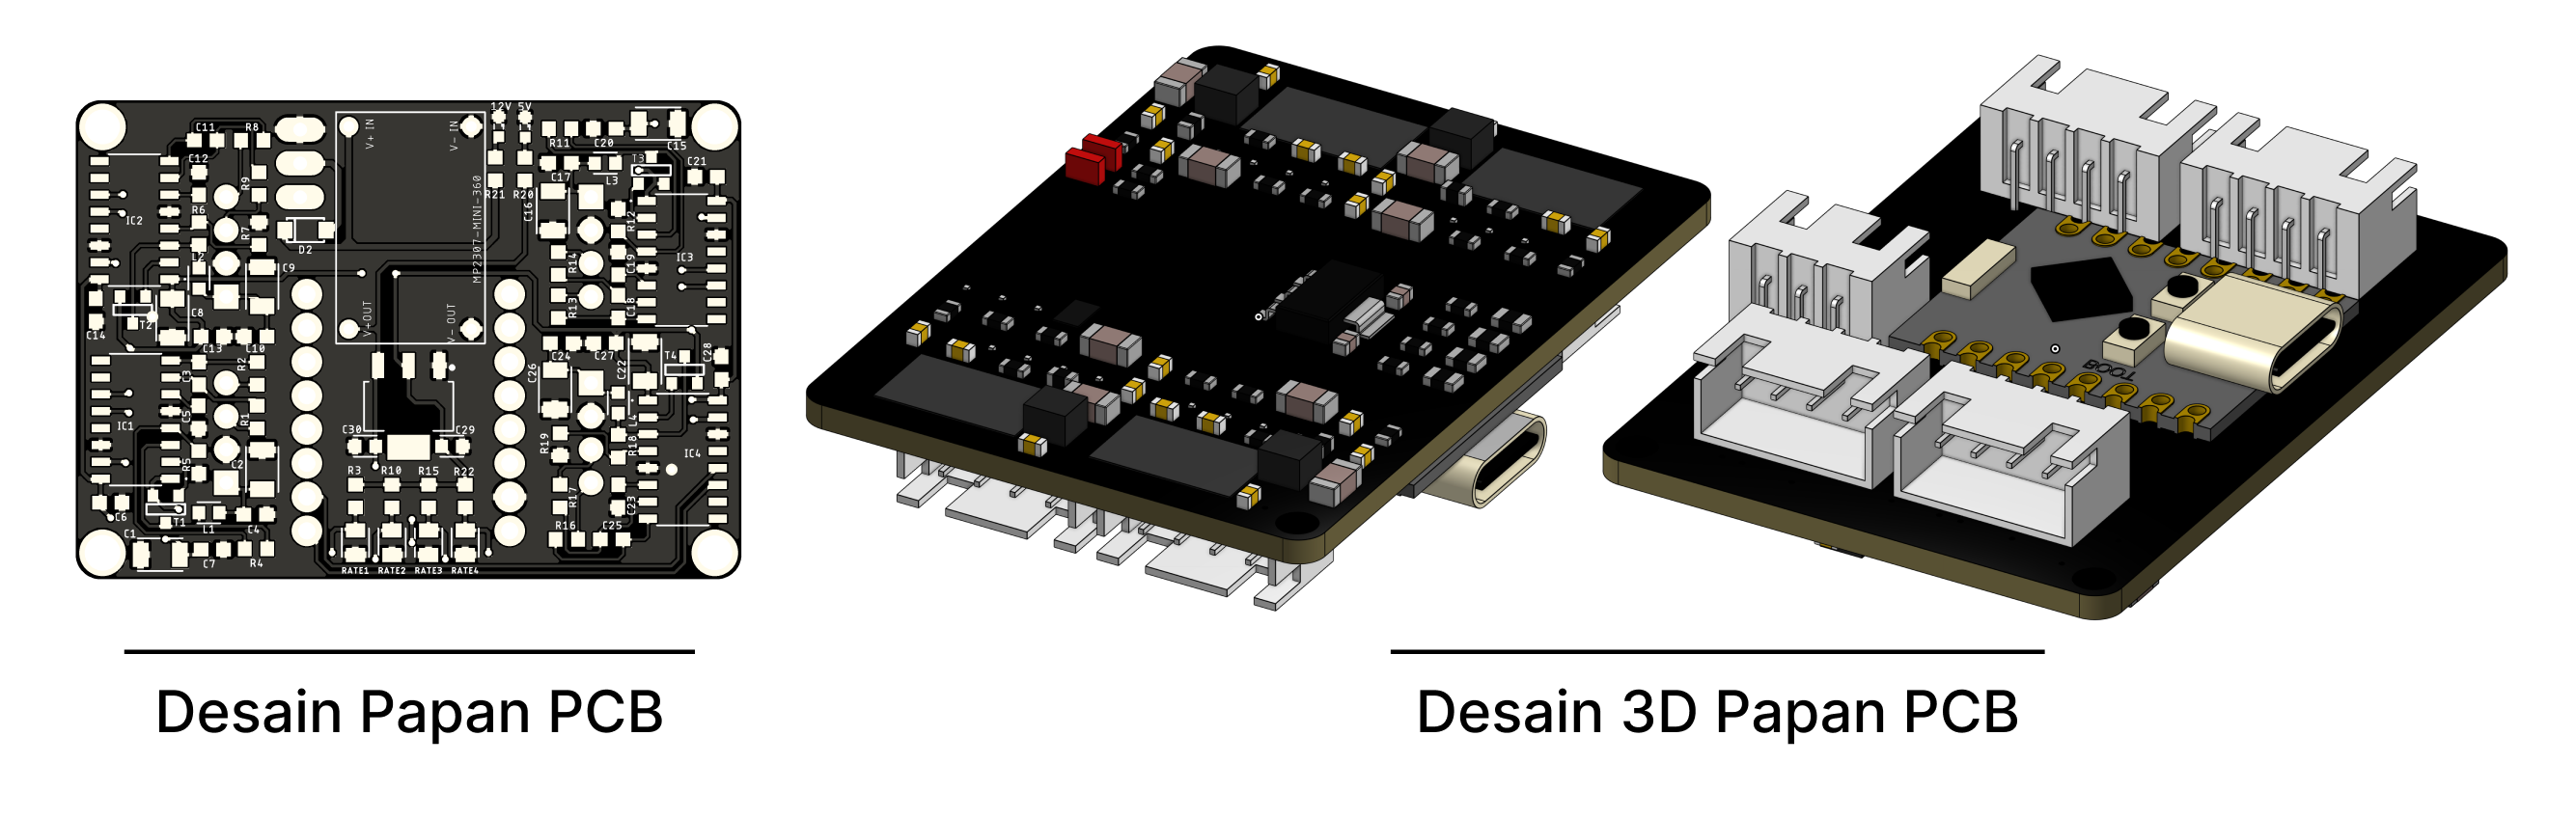
\includegraphics[width=0.4\textwidth]{gambar/Desain_PCB.png}
      \caption{PCB Design}
      \label{fig:Desain_PCB}
    \end{figure}

    \hspace*{1em} Figure \ref{fig:Desain_PCB} shows the PCB layout design to be used on the robot. This PCB has dimensions of 50 x 36 mm with two layers. The top layer contains SMD components, while the bottom layer includes connectors and a microcontroller. This two-layer design allows for more efficient space usage and provides flexibility in component placement.  

    \item Motion Call Algorithm
    \label{subsec:motionalgorithm}

    \hspace*{1em} Before the robot is operated, the program, which also contains pre-made motion data, is uploaded to the non-volatile memory on the microcontroller. The uploaded motion includes data for the servo motors on the robot's upper and lower parts. Next, the robot is operated by inputting a motion index. Each motion index has several frames based on the uploaded motion data. The robot will then execute the movements one by one based on the frames from the inputted motion index.

    \begin{figure} [h]
      \centering
      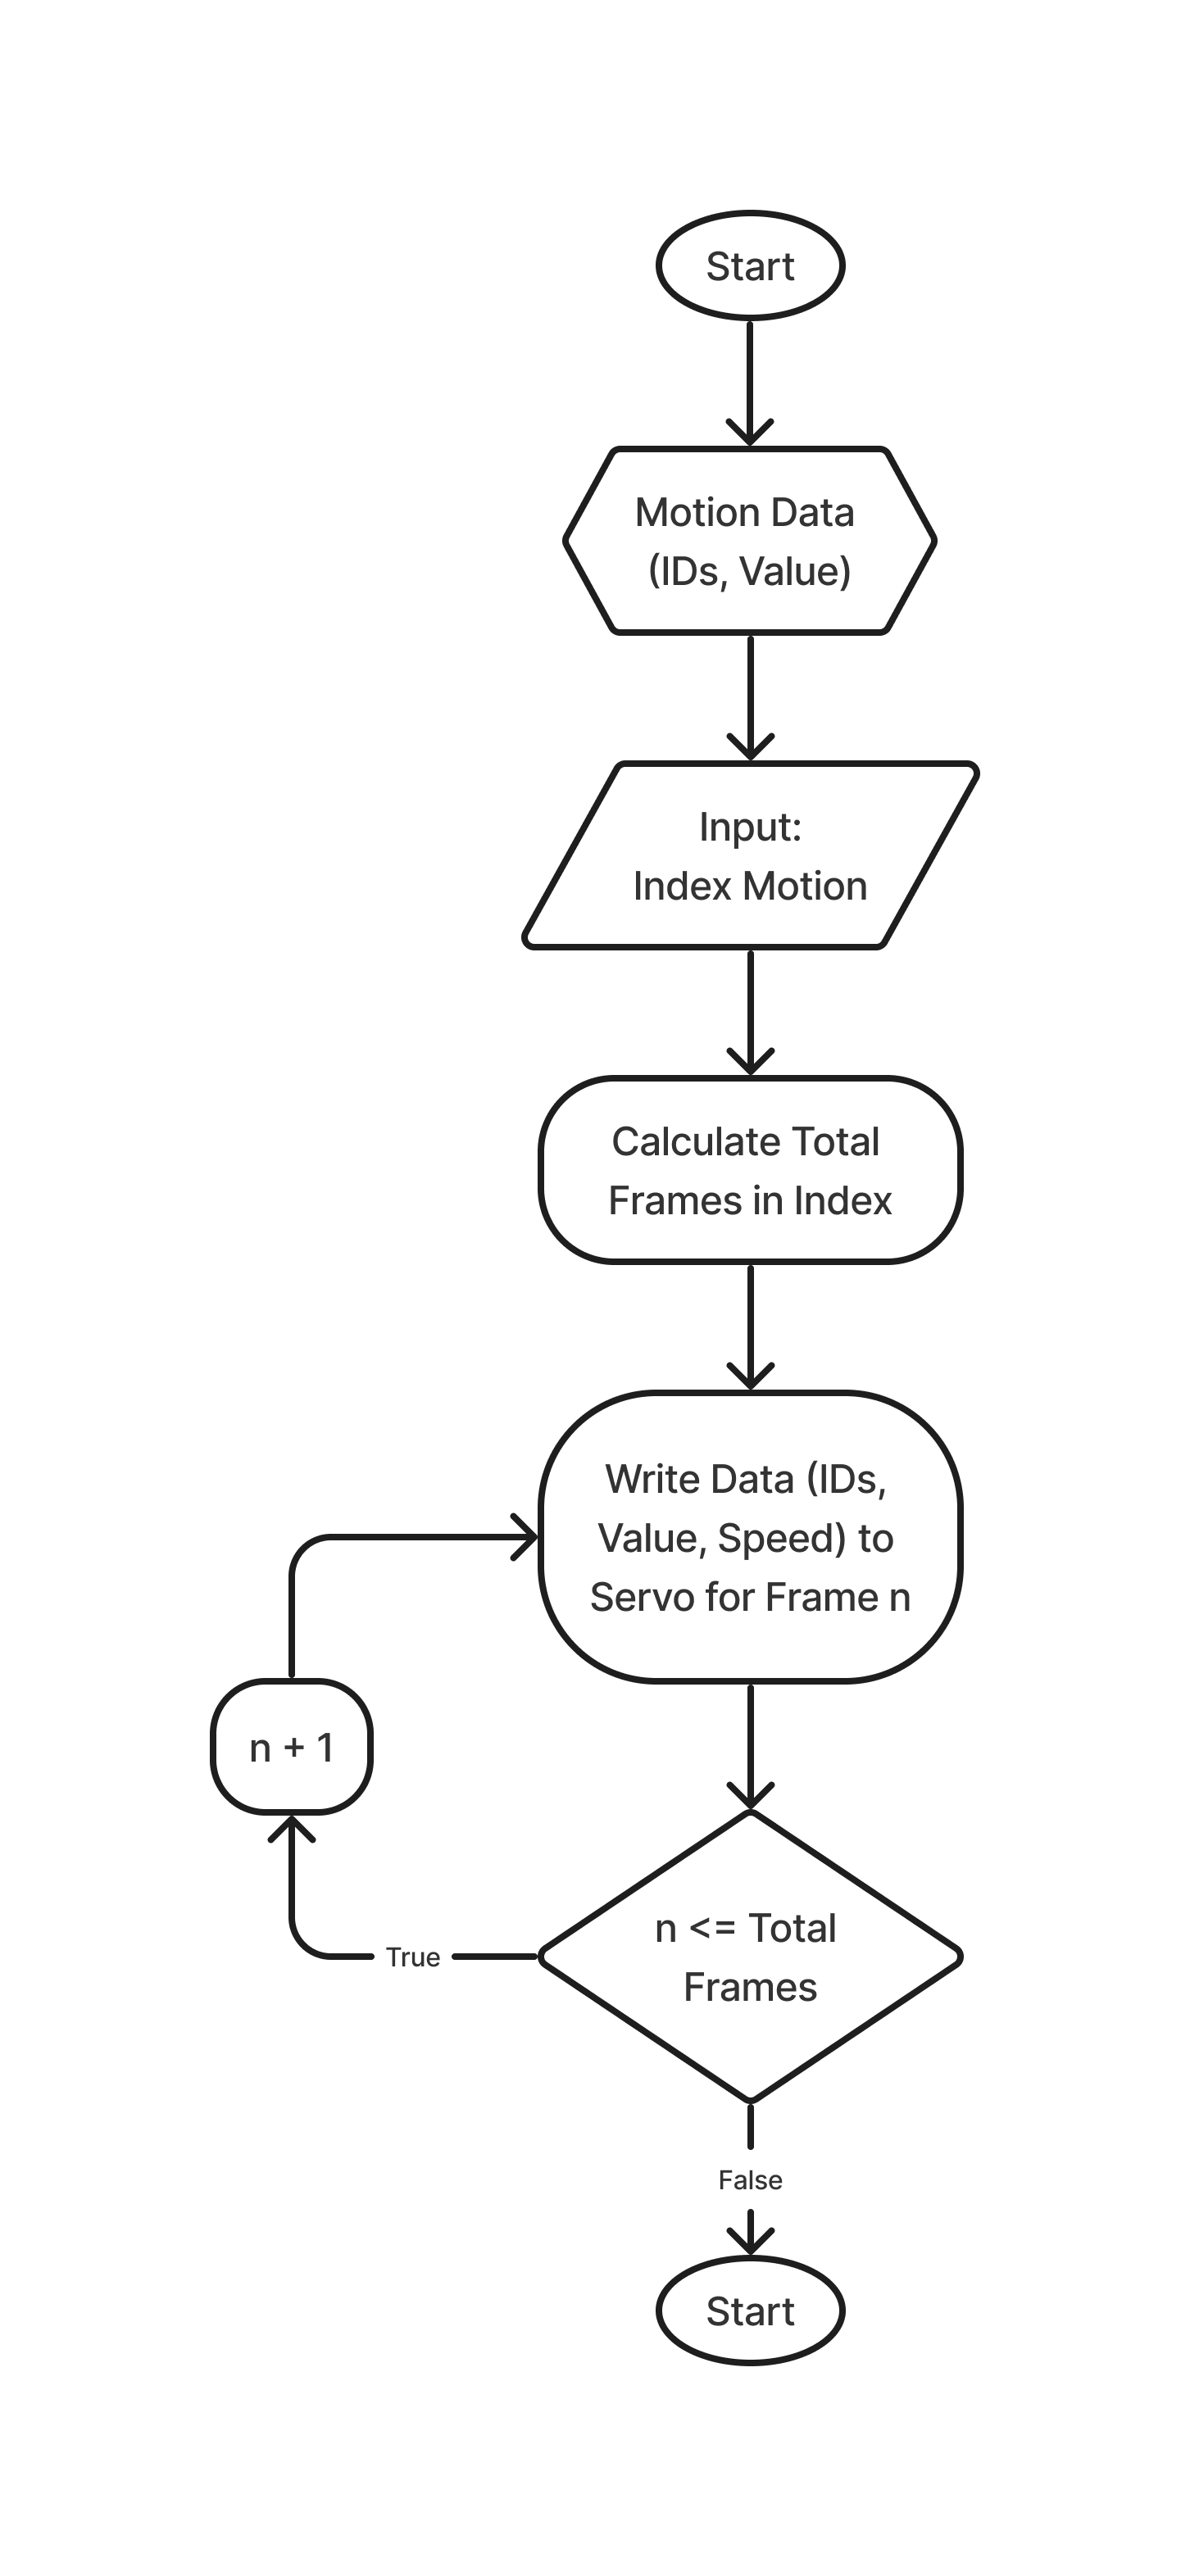
\includegraphics[width=0.3\textwidth]{gambar/flowchart_play_index.png}
      \caption{Flowchart of Program Execution}
      \label{fig:Algoritma_Berjalan}
    \end{figure}

    \item Center of Pressure Calculation for the Robot
    \label{subsec:centerofpressurecalculation}

    \hspace*{1em} The pressure on each load cell is summed using Equation \ref{eq:Total_Force}. The result of this summation is then used to calculate the position of the center of pressure on the x and y axes using Equations \ref{eq:COP_X} and \ref{eq:COP_Y}. In a balanced position, the center of pressure will be at the point (0,0), which is in the middle of the sole. The center of pressure is calculated by summing the pressures towards the center of pressure point on the robot's sole. The range of center of pressure values on the robot's sole is from -1 to 1. The result of the center of pressure calculation is then sent to the main microcontroller that will control the robot's movements. 

    \begin{equation}
      F_{\mathrm{total}} = F_1 + F_2 + F_3 + F_4
      \label{eq:Total_Force}
    \end{equation}

    \begin{equation}
      X_{\mathrm{cop}} = \frac{- F_1 + F_2 - F_3 + F_4}{F_{\mathrm{total}}}
      \label{eq:COP_X}
    \end{equation}

    \begin{equation}
      Y_{\mathrm{cop}} = \frac{F_1 + F_2 - F_3 - F_4}{F_{\mathrm{total}}}
      \label{eq:COP_Y}
    \end{equation}

    \item PID Control Algorithm
    \label{subsec:pidcontrolalgorithm}

    \hspace*{1em} In this research, two PID controls are used: PID Pitch control and PID Roll control. In PID Pitch control, the input is the error value between the center of pressure position on the Y-axis and the set point, while in PID Roll control, the input is the error value between the center of pressure position on the X-axis and the set point. The error value is obtained from the difference between the center of pressure position and the set point as in Equations \ref{eq:Error_Pitch} and \ref{eq:Error_Roll}.

    \begin{equation}
      \mathrm{e}_{\mathrm{pitch}} = \mathrm{SetPoint}_{\mathrm{pitch}} - COP_{\mathrm{Y}}
      \label{eq:Error_Pitch}
    \end{equation}

    \begin{equation}
      \mathrm{e}_{\mathrm{roll}} = \mathrm{SetPoint}_{\mathrm{roll}} - COP_{\mathrm{X}}
      \label{eq:Error_Roll}
    \end{equation}
 
\end{enumerate}
